\chapter{TRABAJOS RELACIONADOS}
Dada la creciente demanda por la generación y apropiamiento de las energías limpias, el estudio de alternativas energéticas basadas en paneles 
solares también ha venido en aumento. Sin embargo, un componente clave para la implementación de una solución de este tipo es analizar de antemano 
las posibles ubicaciones con mayor potencial de generación eléctrica a base de radiación solar. Diversos estudios han consolidado el uso de imágenes 
satelitales de libre acceso como herramientas fundamentales para este propósito. \cite{kaku2009creating} realizó la construcción de mapas solares de alta 
resolución comparando metodologías basadas en imágenes satelitales y modelamiento climático. Para estos modelos de radiación se contemplan condiciones 
propias del terreno como la latitud , el terreno,estación, hora del día y condicione atmosférica(nubes, polvo, polución, vapor de agua y efectos de la montaña)
\begin{figure}[ht]
  \centering 
  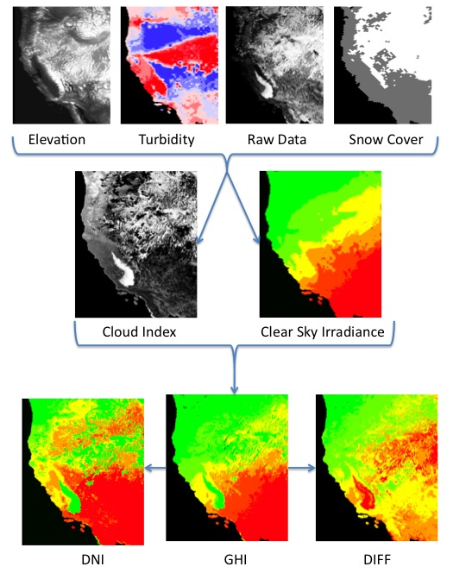
\includegraphics[scale=0.47]{pictures/ER1.png}
  \caption{Diagrama de flujo que representa el cálculo de los valores de irradiancia (Global Horizontal,Directa normal , y Difusa horizontal ) 
  de un área para un área, la fecha dada y ángulo cenital solar.} 
  \label{fig:er1}
\end{figure}
\newpage
\cite{hammer2003solarenergy} desarrolló el método HELIOSAT con el 
objetivo de estimar los niveles de radiación solar a partir de imágenes satelitales geoestacionarias, el método se encuentra implementado 
en un algoritmo que permite separar la irradiación de los componentes atmosférico de la irradiación en nubes para finalmente obtener la 
irradiación superficial.

\begin{figure}[htb]
  \centering 
  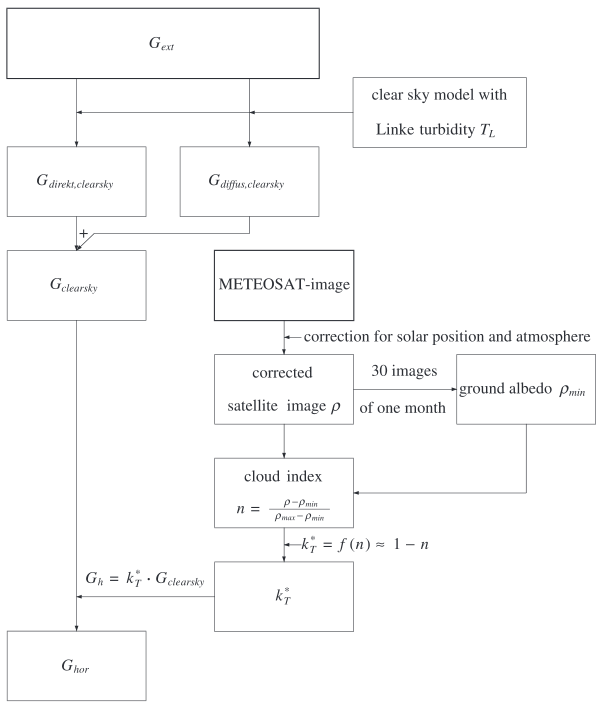
\includegraphics[scale=0.5]{pictures/ER2.png}
  \caption{Descripción general del método HELIOSAT.} 
  \label{fig:er2}
\end{figure}
\newpage
\cite{diagne2012solarirradiation} realiza una recopilación de métodos para la predicción de radiación solar también basados en imágenes por satélite o modelos climáticos, en este estudio 
se contempla la variación de la resolución espacial de la imágen satelital, tipos de sensores utilizados y la escala temporal.
\begin{figure}[htb]
  \centering 
  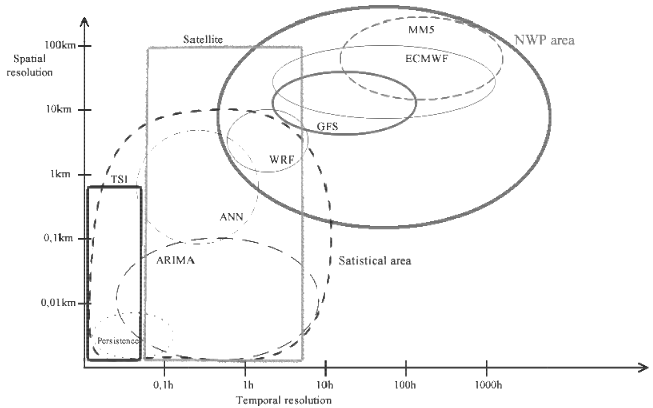
\includegraphics[scale=0.65]{pictures/ER3.png}
  \caption{Clasificación de modelos de predicción basados en resolución espacial de datos y resolución temporal.} 
  \label{fig:er3}
\end{figure}

\cite{wang2012shortterm} obtuvo gran éxito al proponer un nuevo modelo basado en redes neuronales apropiado para pronosticar el potencial solar a corto 
plazo bajo condiciones meteorológicas en constante cambio.

\begin{figure}[htb]
  \centering 
  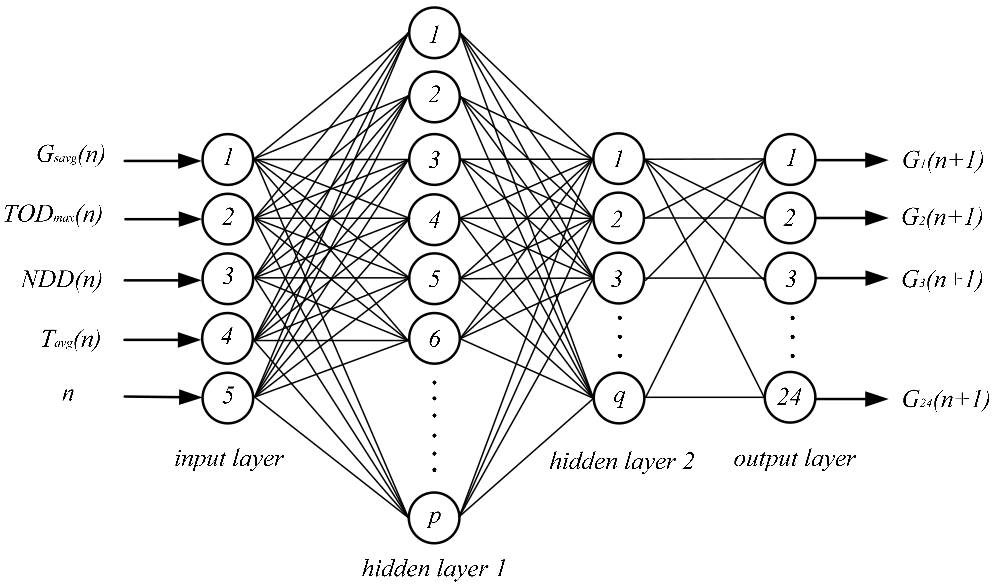
\includegraphics[scale=0.35]{pictures/ER4.png}
  \caption{Modelo de pronóstico ANN utilizando parámetros de características estadísticas.} 
  \label{fig:er4}
\end{figure}
\newpage

\cite{sai2014estimation} señala dos enfoques para obtener radiación neta diaria utilizando los productos de Kalpana VHRR y Oceansat OCM2 mediante el manejo de  la radiación 
de onda larga resultante del flujo de ondas entrantes y salientes, este resultado es computarizado usando la ecuación de Stefan Boltzmann para 
corregir la humedad y la nubosidad,  también se realiza un enfoque basado en la estimación mediante la computación de un cielo despejado con el 
flujo de ondas cortas de radiación que permiten obtener una radiación neta

\begin{figure}[htb]
  \centering 
  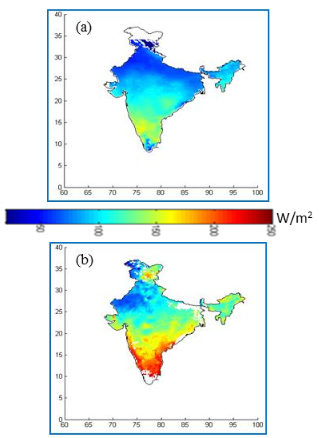
\includegraphics[scale=0.7]{pictures/ER6.png}
  \caption{ Radiación superficial diaria neta de productos de Kalpana VHRR y Oceansat OCM2.} 
  \label{fig:er6}
\end{figure}
\newpage
\cite{mas2011aplicaciones},\cite{ garcia2011evaluacion} generan información de cobertura de suelo, y los métodos que permiten obtener más detalle conservando una fiabilidad 
aceptable sobre la región del Tancítaro, Michoacán y comprende bosques templados y tropicales secos, pastizales y áreas 
de cultivos. Enfocan el estudio en índices de vegetación mediante compuestos espectrales de 8 días e imágenes de reflectancia diarias que 
fueron evaluados por medio de dos metodologías; la máxima verosimilitud y redes neuronales, en cada una de estas se incorporaron 
dos tipos de datos auxiliares. Los resultados muestran que es posible obtener mapas confiables a partir de estos datos de baja resolución 
si se usan categorías generales.

\begin{figure}[htb]
  \centering 
  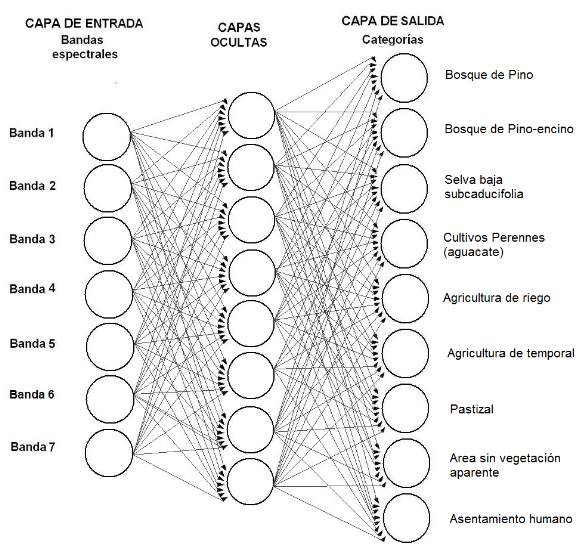
\includegraphics[scale=0.6]{pictures/ER7.png}
  \caption{ Red Neuronal perceptrón multicapa para clasificar una imagen de siete bandas en nueve categorías} 
  \label{fig:er7}
\end{figure}
\newpage
\textbf{\cite{kim2008estimation}} destaca la correlación existente entre la radiación solar incidente en la superficie terrestre y la radiación solar reflejada al espacio; Adicionalmente 
realiza un estudio comparativo en el análisis de  imágenes satelitales MODIS respecto a imágenes satelitales provenientes de SRB, Earth Observing System
(EOS) y Tropical Rainfall Measuring Mission (TRMM), en este estudio se destaca los métodos para estimar la radiación neta obtenida de ondas cortas 
medidas en la superficie.

\newpage
\textbf{\cite{alvarezprocesamiento}} prueban diferentes algorítmos para la detección de aerosoles sobre la superficie terrestre contempladas dentro de imágenes 
satelitales MODIS, implementación del algorithmo Miller sobre las bandas de infrarojo y adicionalmente se realiza una clasificación de los aerosoles detectado.

\begin{figure}[htb]
  \centering 
  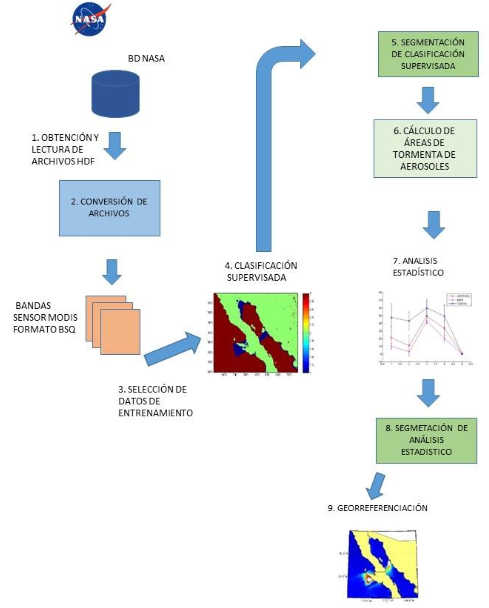
\includegraphics[scale=0.65]{pictures/ER8.png}
  \caption{ Detección de Aerosoles a partir de imágenes satelitales MODIS} 
  \label{fig:er8}
\end{figure}
\newpage
\cite{hashimoto2012prediction} calcula la caída de potencial y fluctuaciones en la generación de energía a partir del seguimiento tridimensional de nubes y su impacto sobre paneles solares.
\begin{figure}[htb]
  \centering 
  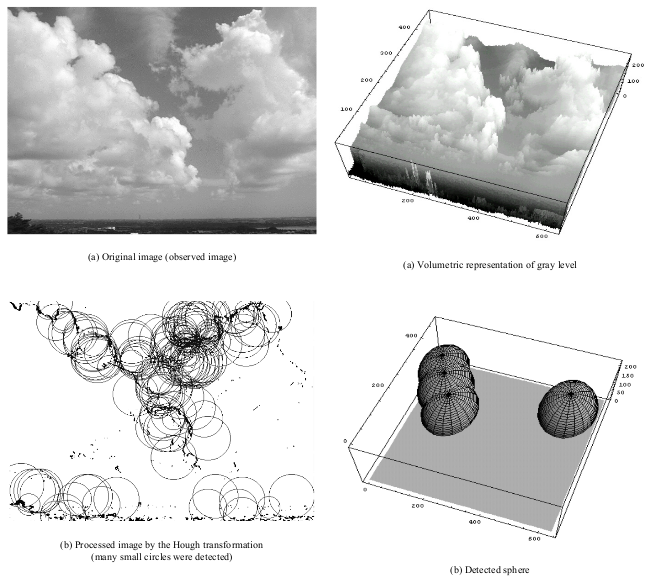
\includegraphics[scale=0.65]{pictures/ER5.png}
  \label{fig:er5}
\end{figure}
